\section{Lezione 2016-10-17}
\subsection{TODO}
% Insert what you need. Any row is associated with the improvment or mistake
% arise. In the first column you can insert what you should resolve or change,
% instead in the second column you may put the section where to apply some
% modification.
\begin{table}[ht]
\begin{center}
\begin{tabular}{|p{\textwidth}|c|}
\hline
\multicolumn{1}{|c|}{\textbf{Miglioramento}} & \textbf{Sezione} \\ \hline
Il processo di diambiguazione \`e manuale, smentire &
\ref{sec:use_ambiguos_grammar} \\ \hline
\end{tabular}
\end{center}
\caption{Tabella miglioramenti}
\label{tab:tab_todo}
\end{table}

\subsection{Usare grammatiche ambigue}
\label{sec:use_ambiguos_grammar}
Tutte le grammatiche usate nella costruzione delle tabella di parsing $LR$
\textbf{dovevano} essere non ambigue. Tuttavia \`e possibile utilizzare anche
grammatiche di origine ambigue, il quale genererebbero conflitti nella tabella,
scegliendone una che va a \textbf{disambiguare} la grammatica (quindi alla fine
si usano sempre grammatiche non ambigue).

L'uso di grammatiche ambigue avvantaggia la scrittura di linguaggi in modi
\textbf{pi\`u naturali}, dove la corrispondente grammatica non ambigua
risulterebbe molto complessa. Con l'uso di grammatiche ambigue si potrebbero
\textbf{eliminare riduzioni non necessarie}.

\subsubsection{Risoluzione conflitti}
Si prenda una grammatica come
$$E \to E+E|E*E|(E)|id$$
con il seguente DFA
\begin{figure}[H]
\centering
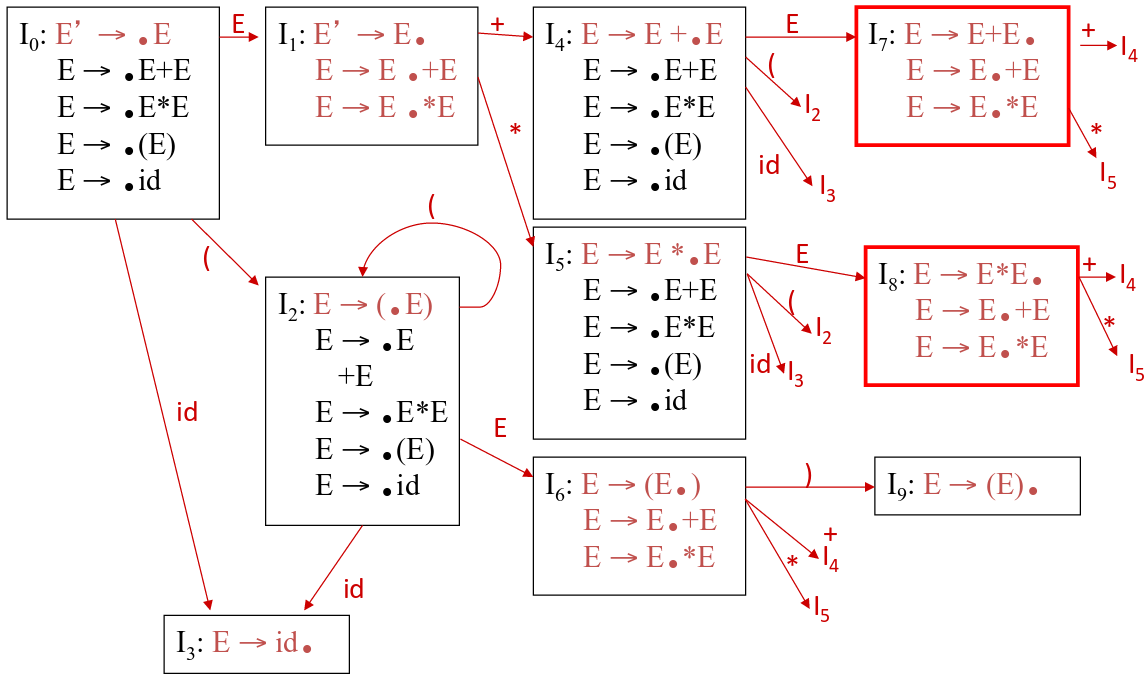
\includegraphics[scale=0.36]{res/image/DFA_ambiguos}
\caption{Automa DFA con grammatica ambigua}
\label{img:DFA_ambiguos}
\end{figure}

Essendo una grammatica ambigua nella tabella di parsing $LR$ sorgeranno dei
conflitti, come in fig.\ref{img:LR_table_ambiguos}.

\begin{figure}[H]
\centering
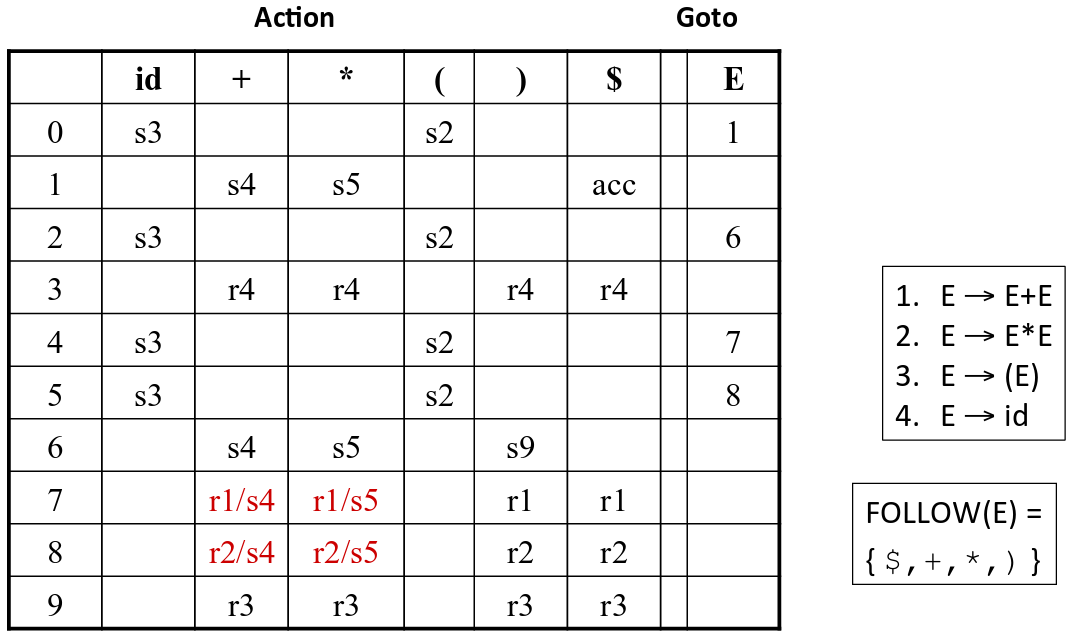
\includegraphics[scale=0.4]{res/image/LR_table_ambiguos}
\caption{Tabella $SRL$ con grammatica ambigua}
\label{img:LR_table_ambiguos}
\end{figure}

La grammatica rappresenta la predecenza/associativit\`a degli operatori. L'
obiettivo \`e \textbf{posticipare/cambiare} questa decisione andando a
risolvere i conflitti emersi.

I conflitti sono riscontrati in due stati:
\paragraph{$I_7$ con conflitti \textit{shift/reduce} per $+$ e $*$}
Allo stato 7 ci si arriva dopo la lettura della sequenza \textbf{id + id}
$$I_0 \xrightarrow{\text{\textbf{E}}} I_1 \xrightarrow{\text{\textbf{+}}}
I_4 \xrightarrow{\text{\textbf{E}}} I_7$$
dopo le dovute riduzioni. Ora bisogna valutare l'azione in base al prossimo
simbolo:
\begin{itemize}
\item quando il token corrente \`e $+$
\begin{align*}
shift   &\implies + \ \text{\`e associativo a destra}   \\
reduce &\implies + \ \text{\`e associativo a sinistra} \Leftarrow
\end{align*}
\item quando il token corrente \`e $*$
\begin{align*}
shift   &\implies * \ \text{ha una precedenza pi\`u alta del} \ + \Leftarrow \\
reduce  &\implies + \ \text{ha una precedenza pi\`u alta di} \ *
\end{align*}
\end{itemize}

\paragraph{$I_8$ con conflitti \textit{shift/reduce} per $+$ e $*$}
Allo stato 8 ci si arriva dopo la lettura della sequenza \textbf{id * id}
$$I_0 \xrightarrow{\text{\textbf{E}}} I_1 \xrightarrow{\text{\textbf{*}}}
I_5 \xrightarrow{\text{\textbf{E}}} I_8$$
dopo le dovute riduzioni. Ora bisogna valutare l'azione in base al prossimo
simbolo:
\begin{itemize}
\item quando il token corrente \`e $*$
\begin{align*}
shift   &\implies * \ \text{\`e associativo a destra}   \\
reduce &\implies * \ \text{\`e associativo a sinistra} \Leftarrow
\end{align*}
\item quando il token corrente \`e $+$
\begin{align*}
shift   &\implies + \ \text{ha una precedenza pi\`u alta di} \  * \\
reduce  &\implies * \ \text{ha una precedenza pi\`u alta del} \ + \Leftarrow
\end{align*}
\end{itemize}

\begin{figure}[H]
\centering
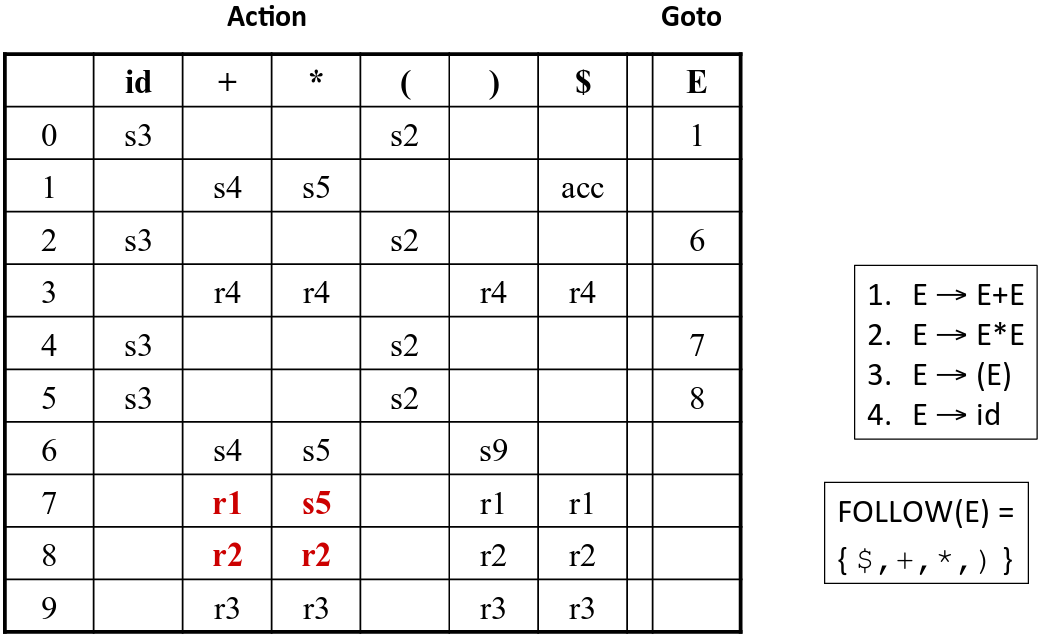
\includegraphics[scale=0.4]{res/image/LR_table_disambiguos}
\caption{Tabella $SRL$ con grammatica disambiguata}
\label{img:LR_table_disambiguos}
\end{figure}

\subsection{Errore recovery nel parsing LR}
Il parser $LR$ individua un errore quando nella lettura di una entry della
tabella di parsing trova una \textit{error entry}. \textbf{Tutte le caselle
vuote} nella tabella \textit{action} sono \textit{error entry} (cosa che non
succederebbe mai consultando la tabella \textit{goto}). L'annuncio dell'errore
dipende dalla tipologia di parser:

\paragraph{Parser in generale ($LR(1)$, $LALR$, $SLR$)}
Non saranno mai inseriti nello stack simboli errati.
\paragraph{$LR(1)$ parser}
Avviser\`a quanto prima non c\`e una valida continuazione della porzione
scansionata dell'input. In particolare \textbf{non eseguira mai una riduzione}
prima di avvisare di un errore.

\paragraph{$SLR$ e $LALR$ parser}
Al contrartio, i due parser \textbf{eseguiranno una serie di riduzioni} prima
di annunciare un errore.

\subsubsection{Panic Mode}
Azioni intraprese:
\begin{enumerate}
\item Scansionamento dall'alto dello stack fino a trovare lo stato $s$ con un
$goto$ su un \textbf{particolare} non-terminale $A$ (lo stack viene liberato
fino al ritrovamento di $s$)
\item Scansionamento dell'input fino a trovare un simbolo $a$ (scartando ogni
simbolo incontrato) che possa seguire legittimamente $A$, generalmente sia nel
$FOLLOW(A$) ma pu\`o anche non funzionare a volte
\item Esegue il push di $(A,goto[s,A])$ e ritorna ad eseguire il parsing
\end{enumerate}

Generalmente $A$ \`e un \textbf{blocco di programma}: \textit{stmt, expr,
block...}; invece $a$ \`e tipicamente o "\textbf{;}" o "\textbf{\}}".

\subsubsection{Phrase-level}
Ogni entry nella tabella di parsing \`e marcata con uno specifico comportamento
a runtime (\textit{error routine}), riflettendo l'errore che l'utente molto
probabilmente far\`a in quel caso. L'azione che si potrebbero compiere \`e
l'inserimento o la cancellazione o entrambe di un simbolo sia dallo stack che
dall'input. Questo andrebbe correggere errori come:
\begin{itemize}
\item operatore mancante
\item parentesi non bilanciate
\end{itemize}

Ad esempio riprendendo la grammatica degli operatori potremmo definire le
seguenti \textit{error routine}:
\paragraph{E1}
Chiamata quando era attesi "\textbf{(}" o "\textbf{id}" ma sono stati trovati
"\textbf{*}", "\textbf{+}" o "\textbf{\$}"
\begin{enumerate}
\item push $id3$ (simbolo "\textbf{id}" seguito dallo stato 3) nello stack
\item stampa "\textit{missing operand}"
\end{enumerate}

\paragraph{E2}
Chiamata quando un "\textbf{)}" inattesa \`e stata trovata
\begin{enumerate}
\item cancella $)$ dall'input
\item stampa "\textit{unbalanced right parenthesis}"
\end{enumerate}

\paragraph{E3}
Chiamata quando era atteso un operatore ma \`e stato trovato "\textbf{id}" o
"\textbf{)}"
\begin{enumerate}
\item push $+4$ nello stack
\item stampa "\textit{missing operator}"
\end{enumerate}

\paragraph{E4}
Chiamata dallo stato 6 quando \`e stata raggiunta la fine dell'input
\begin{enumerate}
\item stampa "\textit{missing right parenthesis}"
\end{enumerate}

Inserendole nella tabella di parsing $LR$, il risultato \`e come appare nella
tabella sottostante.

\begin{figure}[H]
\centering
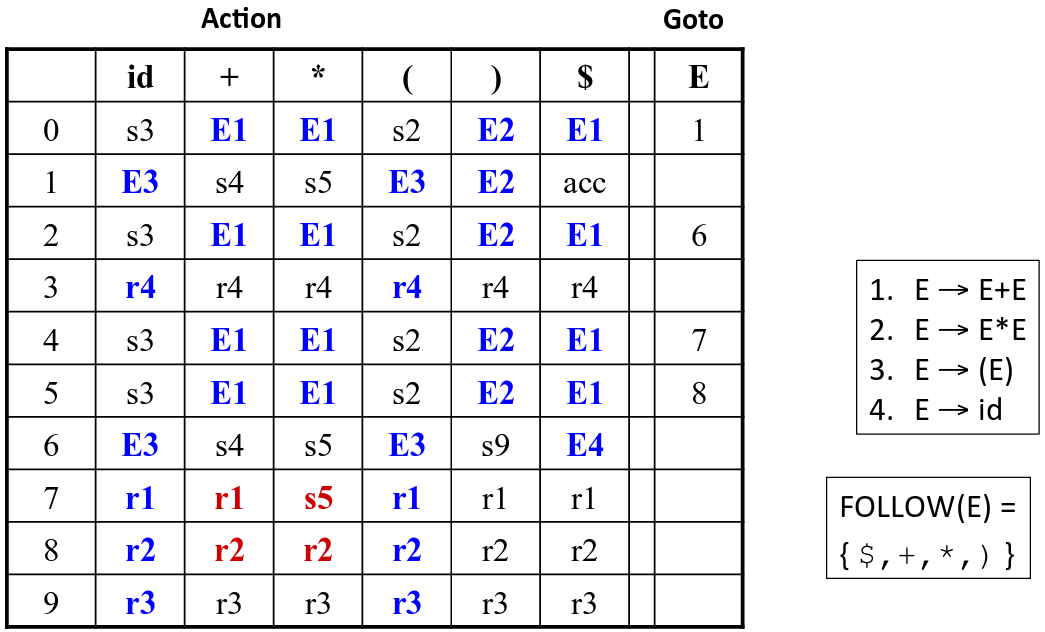
\includegraphics[scale=0.4]{res/image/phrase_recovery_table}
\caption{Tabella $SRL$ con gli \textit{error routine}}
\label{img:phrase_recovery_table}
\end{figure}
